\subsection{Analysis}

\begin{figure}[!ht]
\colorlet{shadecolor}{Mycolor3}
\begin{shaded}
  \centering
    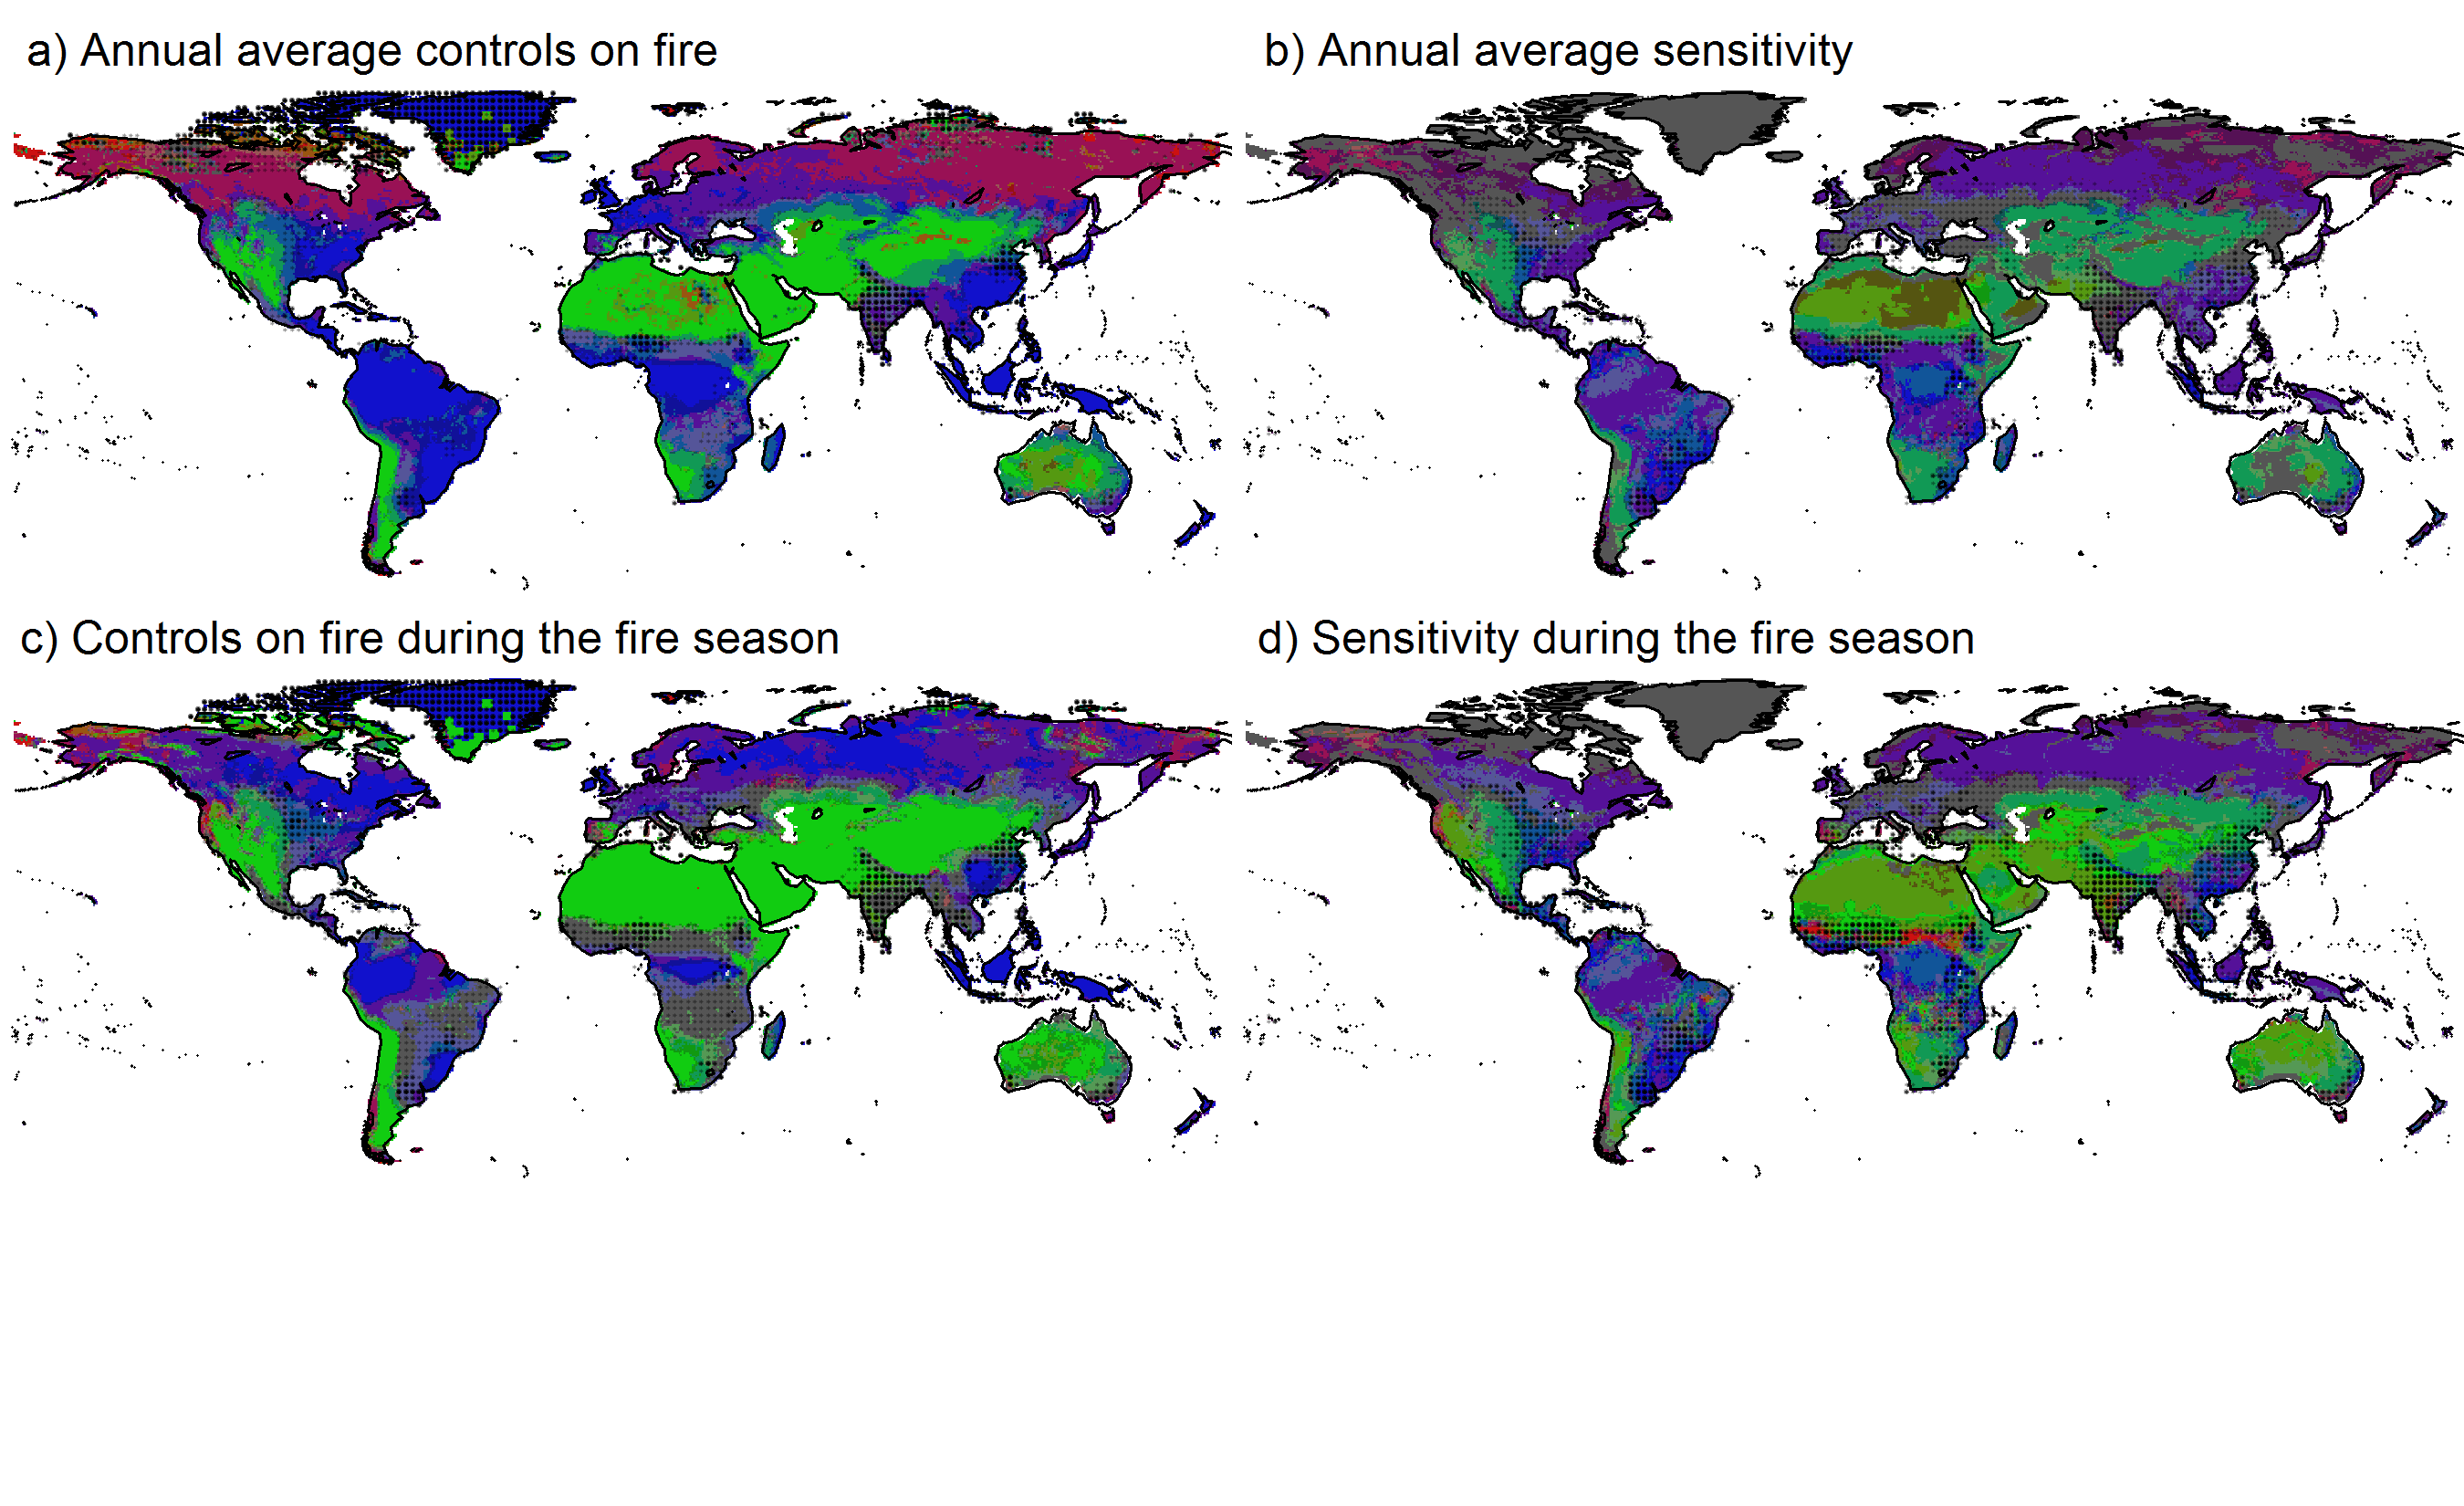
\includegraphics[width=0.9\textwidth]{../figs/limitation_map.png}

  \caption{Limitation and sensitivity.}
  \label{fig:lim_sen_maps}
\end{shaded}
\colorlet{shadecolor}{Mycolor2}
\end{figure}

\subsubsection{Limitation}

The relative importance of each controls was assessed as:

\begin{equation}
    \bar{L_{i, X}} = \frac{L_{i, X}}{\sum_{j} L_{j, X}}
\end{equation}
where $L_{i, X} = 1 - F_{i,X}$ is the individual contribution of each control $i$ for conditions $X$. By definition, $\sum_{i} \bar{L_{i,X}} = 1$, for each location (figures ~\ref{fig:lim_sen_maps} and ~\ref{fig:agu_plot}).


\begin{figure}[!ht]
  \centering
    \includegraphics[width=0.75\textwidth]{../figs/aguplot_Kelleyetal.png}

  \caption{AGU plot.}
  \label{fig:agu_plot}
\end{figure}


\begin{figure}[!ht]
  \centering
    \includegraphics[width=0.67\textwidth]{../figs/moisture_change_for_Amazon_tipping_point.png}

  \caption{Required change in \% fuel moisture content to induce savanna-level fire in the Amazon.}
  \label{fig:amazon}
\end{figure}

\subsubsection{Sensitivity}


\begin{shaded}
    There are two ways I can think of that we could assess sensitivity to each control. We could compare the gradient of each control around the cells current conditions (figure ~\ref{fig:lim_sen_maps}). Alternatively, we could calculate the required change in each control to induce a ``significant'' change in fire regime. The first would be a nice way of classifying different locations, along the same lines as limitations (i.e, Australian Tropical Savanna is xx \% sensitive to changes in fuel load, and yy \% to moisture - see e.g. figure ~\ref{fig:lim_sen_maps}). The second would be harder to normalise across controls, but might be easier to relate to actual changes in climate (i.e, xx $^{\circ}$ increase in temperature would increase fire to expected levels for Savanna - see e.g. figure ~\ref{fig:amazon}; increase in yy \% of agricultural land would reduce fire in non-agricultural land to that expected for forests etc)

\paragraph{options 1}

\begin{equation}
    \bar{\partial L_{i, x}} = \frac{\partial L_{i, x} \cdot \Pi_{j} L_{j, x}}{L_{i, x}}
\end{equation}

where $\partial L_{i, x}$ is the gradient of $L_{i, x}$ relative to the maximum possible gradient of $L_{i}$, occuring when $x = x_{0}$ i.e:

\begin{equation}
    \partial l_{i, x} = \frac{\partial l_{i, x} / \partial X}
                             {\partial l_{i, x_{0}} / \partial x}
\end{equation}

\paragraph{options 2}
for measuring sensitivity is to calculate the change required for a control to alter burnt area enough to induce major alterations in i.e vegetation cover.
For example, assessing amazon risk of fire-induced tipping point. Holding the contribution of ignition, fuel load and land use constant, we could calculate the change in moisture needed to increase burnt area to the level expected for Savanna (roughly 1\% in South America according to \cite{lehmann2011deciphering}).
It would be easy to work out a required change in climate variables (humidity, temperature, ET etc, or any combination of these) required to hit this 'fire tipping point' (figure ~\ref{fig:amazon}).

\end{shaded}
%\pagebreak
\section{Some other results}
\begin{figure}[!ht]
\colorlet{shadecolor}{Mycolor3}
\begin{shaded}
  \centering
    \includegraphics[width=0.8\textwidth]{../figs/HumanImpactMap_small.png}

  \caption{Human impact on burnt area.
            a) Increases in burnt area from human induced fire starts.
            b) Changes in burnt area from human fire starts and suppression.}
    \label{fig:human_impact}
\end{shaded}
\colorlet{shadecolor}{Mycolor2}
\end{figure}

\begin{figure}
\colorlet{shadecolor}{Mycolor3}
\begin{shaded}
  \centering
    \includegraphics[width=0.67\textwidth]{../figs/cropland_noCrop_impact.png}

  \caption{The impact of cropland on burnt area in non-cropland within the same grid cell.}
\end{shaded}
\colorlet{shadecolor}{Mycolor2}
\end{figure}
